% Source: Wald GR, physical PDF p. 407
%         (printed p. 394).
% Coverage: A spacetime flat outside the compact region K.
% Figures/tables/footnotes: Figure 14.1; no tables or footnotes.
% Status: source-reviewed and compile-clean.
% Uncertainties: none.

\begingroup
\renewcommand{\thefigure}{14.1}
\begin{figure}[htbp]
  \centering
  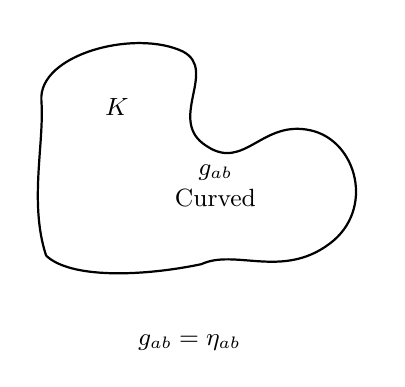
\begin{tikzpicture}[x=1cm,y=1cm,font=\small,line cap=round,line join=round]
    \draw[thick]
      (-1.70,-1.25)
      .. controls (-1.92,-.58) and (-1.72,.18) .. (-1.76,.72)
      .. controls (-1.80,1.31) and (-.56,1.63) .. (.04,1.34)
      .. controls (.49,1.10) and (-.18,.46) .. (.34,.14)
      .. controls (.82,-.18) and (1.04,.48) .. (1.66,.34)
      .. controls (2.25,.21) and (2.48,-.67) .. (1.90,-1.10)
      .. controls (1.30,-1.55) and (.70,-1.16) .. (.27,-1.36)
      .. controls (-.50,-1.52) and (-1.40,-1.54) .. (-1.70,-1.25)
      -- cycle;
    \node at (-.80,.64) {\(K\)};
    \node[align=center] at (.45,-.36) {\(g_{ab}\)\\Curved};
    \node at (.12,-2.35) {\(g_{ab}=\eta_{ab}\)};
  \end{tikzpicture}
  \caption{A spacetime diagram of a spacetime \((\mathbb R^4,g_{ab})\) which is
  isometric to Minkowski spacetime \((\mathbb R^4,\eta_{ab})\) outside of a
  compact region \(K\).}
  \label{fig:14.1}
\end{figure}
\endgroup
